\begin{frame}
  \frametitle{General inner products} 
  %% \framesubtitle{}
  
  \begin{itemize}
  \item Can we also introduce geometric notions such as angles and orthogonality
    for other metrics, e.g.\ the Manhattan distance?
    \begin{itemize}
    \item[\hand] norm must be derived from appropriate inner product
    \end{itemize}
    \pause\gap
  \item General \h{inner products} are defined by
    \[ 
    \sprod{\vu}{\vv}_B \coloneq (\vx')^T \vy' = x'_1 y'_1 + \dots + x'_ y y'_n 
    \] 
    wrt.\ non-Cartesian basis $B$ ($\vu \equiv_B \vx'$, $\vv \equiv_B \vy'$)%
    \pause\gap
  \item $\sprod{\cdot}{\cdot}_B$ can be expressed in standard coordinates
    $\vu\equiv_E \vx$, $\vv \equiv_E \vy$ using the transformation matrix
    $\mathbf{B}$:
    \begin{align*}
      \sprod{\vu}{\vv}_B &= (\vx')^T \vy' 
      = \bigl( \mathbf{B}^{-1} \vx \bigr)^T \bigl( \mathbf{B}^{-1} \vy \bigr) \\
      &= \vx^T (\mathbf{B}^{-1})^T \mathbf{B}^{-1} \vy \eqcolon \vx^T \mathbf{C} \vy
    \end{align*}
  \end{itemize}
\end{frame}

\begin{frame}
  \frametitle{General inner products} 
  %% \framesubtitle{}
  
  \begin{itemize}
  \item The coefficient matrix $\mathbf{C} \coloneq (\mathbf{B}^{-1})^T
    \mathbf{B}^{-1}$ of the general inner product is \h{symmetric}
    \[
    \mathbf{C}^T = (\mathbf{B}^{-1})^T ((\mathbf{B}^{-1})^T)^T =
    (\mathbf{B}^{-1})^T \mathbf{B}^{-1} = \mathbf{C}
    \]
    \pause
    and \h{positive definite}
    \[
    \vx^T \mathbf{C} \vx 
    = \bigl( \mathbf{B}^{-1} \vx \bigr)^T \bigl( \mathbf{B}^{-1} \vx \bigr)
    = (\vx')^T \vx' \geq 0
    \]
    \pause
  \item It is (relatively) easy to show that every positive definite and
    symmetric bilinear form can be written in this way.
    \begin{itemize}
    \item[\hand] i.e.\ every norm that is derived from an inner product can be
      expressed in terms of a coefficient matrix $\mathbf{C}$ or basis $B$
    \end{itemize}
  \end{itemize}
\end{frame}

\begin{frame}
  \frametitle{General inner products} 
  %% \framesubtitle{}
  
  \begin{columns}[T]
    \begin{column}{50mm}
      An example:
      \begin{itemize}\gap
      \item $\vb[1] = (3,2)$, $\vb[2] = (1,2)$
      \item \(
        \mathbf{B} = \begin{bmatrix}
          3 & 1 \\ 2 & 2
        \end{bmatrix} \)
      \item \(
        \mathbf{B}^{-1} = \begin{bmatrix}
          \frac12 & -\frac14 \\ -\frac12 & \frac34
        \end{bmatrix} \)
      \item \(
        \mathbf{C} = \begin{bmatrix}
          .5 & -.5 \\ -.5 & .625
        \end{bmatrix} \)
      \item Graph shows \hh{unit circle} of the inner product $\mathbf{C}$, i.e.\
        points $\vx$ with \[ \vx^T \mathbf{C} \vx = 1 \]
      \end{itemize}
    \end{column}
    \begin{column}{50mm}
      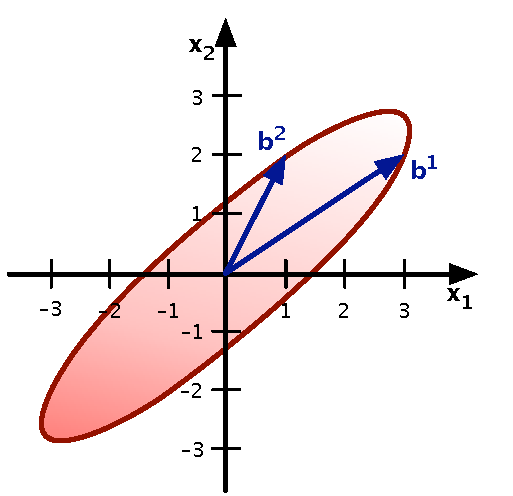
\includegraphics[width=50mm]{img/2_inner_product_1}
    \end{column}
  \end{columns}
\end{frame}

\begin{frame}
  \frametitle{General inner products} 
  %% \framesubtitle{}
  
  \begin{columns}[T]
    \begin{column}{50mm}
      \begin{itemize}\gap
      \item $\mathbf{C}$ is a symmetric matrix
      \item There is always an orthonormal basis such that $\mathbf{C}$ has
        diagonal form
      \item ``Standard'' dot product with additional scaling factors
        (wrt.\ this orthonormal basis)
      \item Intuition: unit circle is a squashed and rotated disk
      \end{itemize}
    \end{column}
    \begin{column}{50mm}
      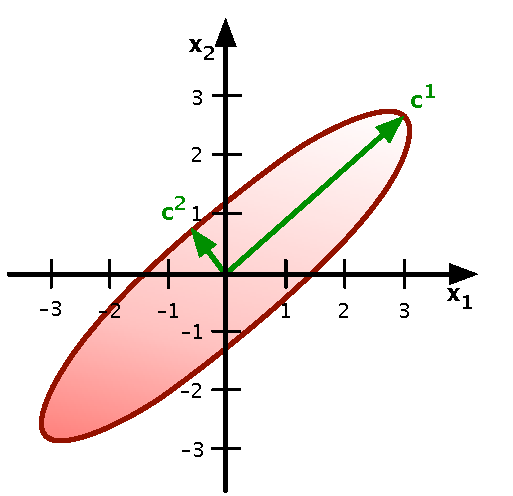
\includegraphics[width=50mm]{img/2_inner_product_2}
    \end{column}
  \end{columns}
  \begin{itemize}
  \item<2->[\So] Every ``geometric'' norm is equivalent to the Euclidean norm
    except for a rotation and rescaling of the axes
  \end{itemize}
\end{frame}

%%% Local Variables: 
%%% mode: latex
%%% TeX-master: "../../workspace"
%%% End: 
